\documentclass[12pt]{article}
\usepackage[utf8]{inputenc} % fonts and characters and stuff
\usepackage[a4paper, margin=3cm]{geometry} % margin size and stuff
\usepackage{amsmath} % maths and stuff
\usepackage{graphicx} % figures and stuff
\usepackage[colorlinks=true, allcolors=blue]{hyperref} % links and stuff
\usepackage{color}
\usepackage{listings}
\usepackage{amsfonts}
\usepackage{amsmath}
\usepackage{amssymb}
\usepackage{enumitem}
\usepackage{fancyhdr}
\usepackage{sectsty}
\sectionfont{\centering}

\lhead{CS 511 Formal Methods, Fall 2024}
\rhead{Instructor: Assaf Kfoury}


\newcommand{\leancopilot}{\texttt{LeanCopilot} }
\newcommand{\llmstep}{\texttt{LLMStep} }
\definecolor{keywordcolor}{rgb}{0.7, 0.1, 0.1}   % red
\definecolor{tacticcolor}{rgb}{0.0, 0.1, 0.6}    % blue
\definecolor{commentcolor}{rgb}{0.4, 0.4, 0.4}   % grey
\definecolor{symbolcolor}{rgb}{0.0, 0.1, 0.6}    % blue
\definecolor{sortcolor}{rgb}{0.1, 0.5, 0.1}      % green
\definecolor{attributecolor}{rgb}{0.7, 0.1, 0.1} % red
\def\lstlanguagefiles{lstlean.tex}
\lstset{language=lean}


% Title
\title{\bf{Large Language Models For Automatic Theorem Proving: A Study Using Lean4}}
\author{Lucas Miguel Tassis}
\date{December 13, 2024}

% Begin configs
\begin{document}
\maketitle
\thispagestyle{fancy}

\renewcommand{\contentsname}{Table of Contents}
\tableofcontents

\newpage
\section{Introduction}
Large Language Models (LLMs) have shown significant potential for automatic theorem proving using proof assistants like Coq, Isabelle, and Lean \cite{neurips}. However, automatic theorem proving is still a challenging task for machine learning models, since it requires rigorous formal proofs that can have their correctness verified. This is especially difficult in language models, since LLMs are particularly prone to ``hallucinating'', \emph{i.e.}, generating outputs that are inaccurate and inconsistent with their training data.

Some recent works in the literature try to tackle the challenge of using LLMs in automatic theorem proving in a more consistent and accurate manner. More specifically, for the interactive theorem proving tool Lean,
two tools have appeared in the literature: \llmstep \cite{llmstep} and \leancopilot \cite{leancopilot}.

Both \llmstep and \leancopilot were designed to assist humans in proving theorems using Lean4. These tools help the proving process by suggesting  proof steps, and in the particular case of \leancopilot, selecting premises and even generating full proofs. 

In this project, we investigate the use of LLMs in automatic theorem proving in Lean using both \llmstep and \leancopilot. First, we present both tools and how they work. Then, we perform experiments using both tools to evaluate the performance of LLM-based theorem provers in a variety of settings. 

The remainder of this document is organized as follows: Section \ref{sec:tools} presents and briefly describes both \llmstep and \leancopilot. Section \ref{sec:experiments} presents experiments conducted using both tools. Section \ref{sec:conclusion} presents some conclusions from the experiments performed in this project. Finally, Section \ref{sec:futurework} presents some ideas for future work.

\section{Tools for Automatic Theorem Proving} \label{sec:tools}

In this section, we present a brief introduction on the tools that will be used in this project. First we present the LLMStep, then we present the LeanCopilot tool. 

\subsection{\llmstep}
\llmstep \cite{llmstep} is a tool for suggesting proof steps (\emph{i.e.} tactics) in the Lean proof assistant. The tool works by sending the user's proof state to a server that hosts a language model. The server handles the query made in the Lean4 script and relays back the answer of the language model. The language model itself is trained to produce the next tactic given the current state of the proof. More specifically, the language model is trained to answer the following prompt:

\begin{center}
    \texttt{[GOAL] tactic\_state [PROOFSTEP] next\_tactic}
\end{center}

Therefore, by inputting the goal and current tactic state, the model produces a suggestion for the next tactic. The default language model used by \llmstep is the \texttt{Pythia 2.8b} fine-tuned on \texttt{(state, next\_tactic)} examples from Mathlib.

The \llmstep tool works in Lean similarly to a tactic: if you call \texttt{llmstep <prefix>} within a proof, it will return suggestions of proofs steps using the prefix tactic. Moreover, it can also suggest tactics without a prefix, by using \texttt{llmstep ""}. Figure \ref{fig:tools-llmstep} presents a diagram of the \llmstep tool.

\begin{figure}[h]
  \centering
  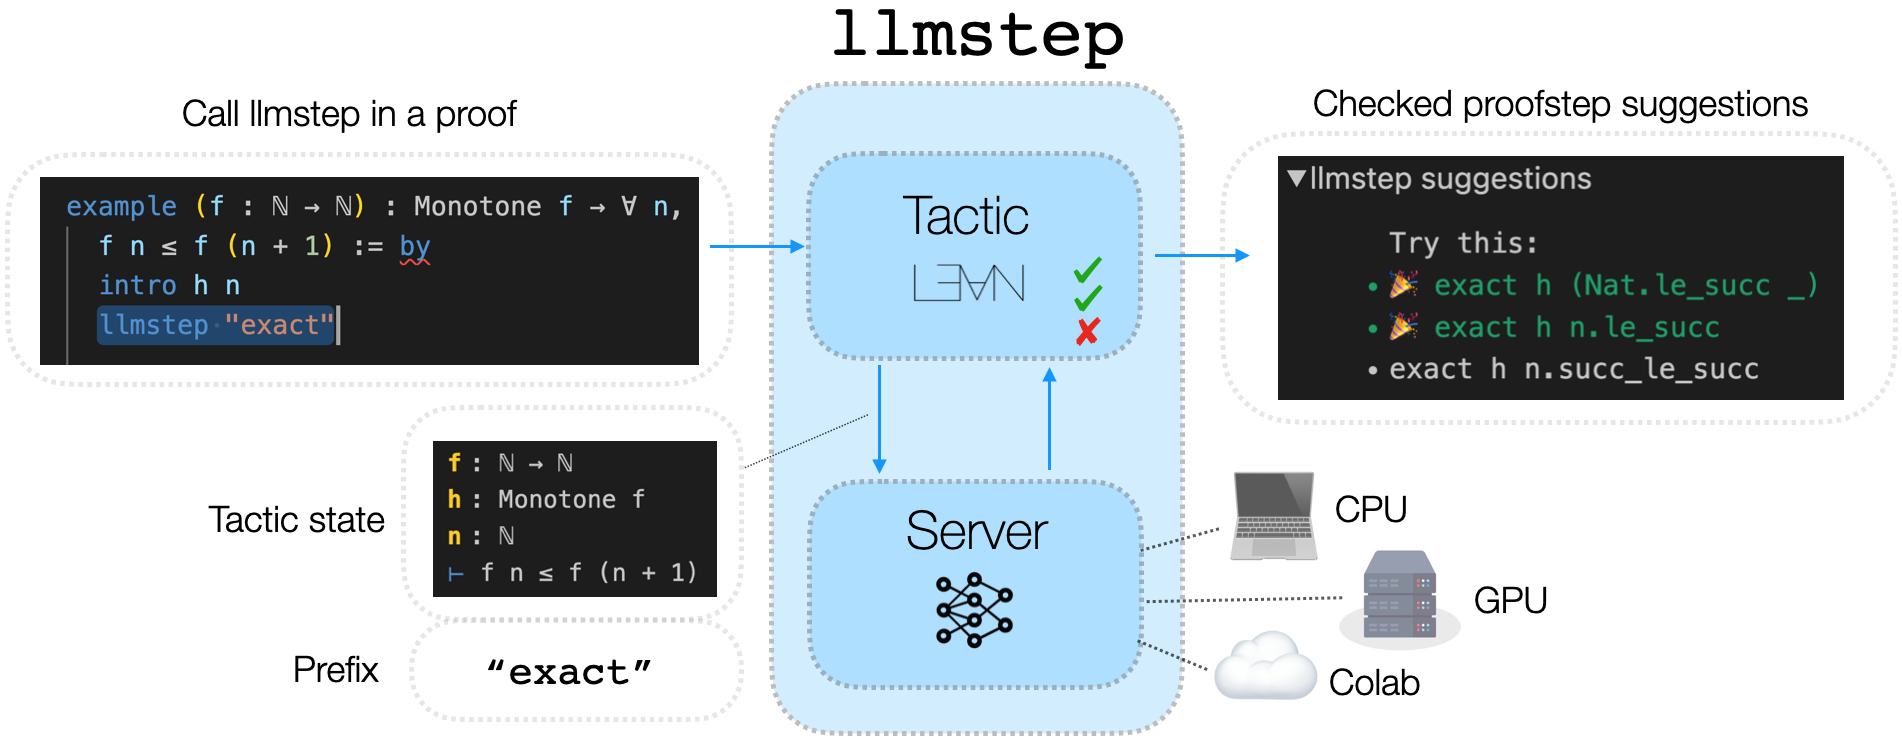
\includegraphics[width=\linewidth]{figures/llmstep.png}
  \caption{Illustration of the \llmstep tool. Source: \cite{llmstep}}
  \label{fig:tools-llmstep}
\end{figure}

In comparison with the \leancopilot tool, this tool is significantly less powerful, since it only gives a single proof suggestion. However, we can imagine that a full proof could be created by calling several proof suggestions (some brief experiments will be conducted on this). Finally, the paper states that \textit{``the tool is agnostic to the choice of language model, learning framework and evaluation framework''}. Therefore, the subparts of the tool can be replaced if the user has more or less computational resources for example.

\subsection{\leancopilot}

The \leancopilot tool \cite{leancopilot} was designed by a group of researchers that developed a number of tools for extracting data from Lean, and also training machine learning models. All the tools developed by the group can be found under the name: LeanDojo\footnote{https://leandojo.org/}. The \leancopilot tool is a significantly more powerful tool than the \llmstep one, since not only suggest proof steps but also premise selection and even full proofs.

Similar to the functioning of \llmstep, \leancopilot is also called as a tactic inside the Lean code, however we have three tactics:

\begin{enumerate}[label=(\arabic*)]
  \item \texttt{suggest\_tactics}: this tactic suggests a single next tactic.
  \item \texttt{select\_premises}: this tactic suggests which premises might be more relevant to finish the goal.
  \item \texttt{proof\_search}: this tactic attempts to create a full proof. It combines LLM-generated proofs with the \texttt{aesop} Lean tactic.
\end{enumerate}

The tactic \texttt{suggest\_tactics} works similarly to the \llmstep tool, \emph{i.e.}, given the goal and the state, the language model has to produce a suggestion for the next tactic. Additionally, it checks if the suggestion candidate would: lead to errors; lead to no errors, however cannot finish the goal; and finish the proof. 

The tactic \texttt{proof\_search} works by combining the previous LLM-based tactic suggestion with the tool \texttt{aesop} . \texttt{aesop} is a rule-based proof search tool (\emph{i.e.} it does not use any LLM) already available in Lean4. It builds a search tree and expands it by applying tactics to the most promising unexpanded nodes. The proof search is successful when it finds a path from the root to the goal. In \texttt{aesop}, the tactics for expanding are drawn from a set called \textit{rule set}. This rule set is fixed and can be chosen by the user (but it is fixed for every proof). \leancopilot uses the \texttt{suggest\_tactics} to expand the rule set in a dynamic manner. Therefore, the authors argue that this addition makes \texttt{aesop} \textit{substantially more flexible} than the regular version. 

In our work, we mainly explore the use of \texttt{proof\_search} in several kinds of proof, trying to understand where it succeeds and where it fails. Figure \ref{fig:tools-leancopilot} presents a diagram of the \leancopilot tool.

\begin{figure}[h]
  \centering
  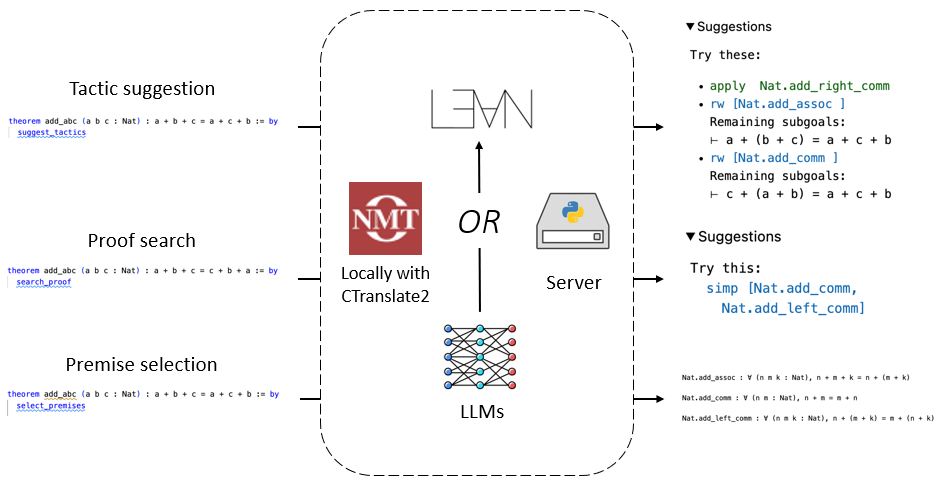
\includegraphics[width=\linewidth]{figures/leancopilot.png}
  \caption{Illustration of the \leancopilot tool. Source: \cite{leancopilot}}
  \label{fig:tools-leancopilot}
\end{figure}

\section{Experiments} \label{sec:experiments}
In this section, we present the experiments conducted to evaluate the two LLMs tools. First, we present the results of full proof searches using \leancopilot, evaluating the performance of the model in a variety of proof types. Then, we make a small study for evaluating step suggestions by \llmstep. Finally, we attempt to finish some incomplete \leancopilot proofs with step suggestions by \llmstep. All the examples used in these experiments were from the book The Mechanics of Proof by Professor Heather Macbeth\footnote{https://hrmacbeth.github.io/math2001/}. The experiments compare the automatic generated proof with a human one. The large majority of the human proofs were created by me for the class homework and lab assignments. However, a few of them were from the MoP example section (and the proof is already presented there).

\subsection{Proof Search with \leancopilot}
In the first part of the experiments, we evaluate the performance of the \leancopilot tool in different kinds of proofs. Each subsection presents an example where the tool found a proof, and most also presents one where it failed. Additionally, we try to understand why the tool failed to find a proof, based on the examples.

%%%%%%%%%%%%%%%%%%%%%%%%%%%%%%%%%%%%%%%%%%%%%%%%%%%%%%%%%%%%%%%%%%%%%%%%%%%
\subsubsection{Proofs by Calculation}
First, let us consider some proofs using only calculations. These proofs are rather easy to prove using \texttt{calc} blocks. The first example is the following:

\begin{minipage}{0.495\textwidth}
  \begin{lstlisting}[title={Human proof}]
  -- Example 1.3.1
  example {a b : ℤ} (h1 : a = 2 * b + 5) (h2 : b = 3) : a = 11 := by
    calc
      a = 2 * b + 5 := by rw [h1]
      _ = 2 * 3 + 5 := by rw [h2]
      _ = 11 := by ring
  \end{lstlisting}
\end{minipage}
\vline
\begin{minipage}{0.495\textwidth}
  \begin{lstlisting}[title={\leancopilot proof}]
  -- Example 1.3.1
  example {a b : ℤ} (h1 : a = 2 * b + 5) (h2 : b = 3) : a = 11 := by
    -- search_proof
    subst h2 h1
    simp_all only [Int.reduceMul, Int.reduceAdd]
  \end{lstlisting}
\end{minipage}

Notice that the tool found an answer without using a \texttt{calc} block. Next, an example where it failed:

\begin{minipage}{0.495\textwidth}
  \begin{lstlisting}[title={Human proof}]
  -- Example 1.3.4
  example {w : ℚ} (h1 : 3 * w + 1 = 4) : w = 1 := by
  calc
    w = ((3 * w + 1) / 3) - (1 / 3) := by ring
    _ = (4 / 3) - (1 / 3) := by rw [h1]
    _ = 1 := by ring
  \end{lstlisting}
\end{minipage}
\vline
\begin{minipage}{0.495\textwidth}
  \begin{lstlisting}[title={\leancopilot proof}]
  -- Example 1.3.4
  example {w : ℚ} (h1 : 3 * w + 1 = 4) : w = 1 := by
    -- search_proof
    sorry
  \end{lstlisting}
\end{minipage}

In this second example, the tool failed to find a proof despite the example also being rather simple. The difference, is that in the second example, we had to manipulate the expression a bit more, instead of only rewriting the hypothesis (like in the first case). 


%%%%%%%%%%%%%%%%%%%%%%%%%%%%%%%%%%%%%%%%%%%%%%%%%%%%%%%%%%%%%%%%%%%%%%%%%%%
\subsubsection{Inequalities}
Next, we evaluate the tool for proofs using inequalities. Similar to the proofs by calculation, these proofs only involve \texttt{calc} blocks, and are rather simple. The first example is the following:

\begin{minipage}{0.495\textwidth}
  \begin{lstlisting}[title={Human proof}]
  -- Example 1.4.1
  example {x y : ℤ} (hx : x + 3 ≤ 2) (hy : y + 2 * x ≥ 3) : y > 3 := by
    calc
      y = y + 2 * x - 2 * x := by ring
      _ ≥ 3 - 2 * x := by rel [hy]
      _ = 9 - 2 * (x + 3) := by ring
      _ ≥ 9 - 2 * 2 := by rel [hx]
      _ > 3 := by numbers
  \end{lstlisting}
\end{minipage}
\vline
\begin{minipage}{0.495\textwidth}
  \begin{lstlisting}[title={\leancopilot proof}]
  -- Example 1.4.1
  example {x y : ℤ} (hx : x + 3 ≤ 2) (hy : y + 2 * x ≥ 3) : y > 3 := by
    -- search_proof  
    simp_all only [ge_iff_le, gt_iff_lt]
    omega
  \end{lstlisting}
\end{minipage}

Notice that the tool finds a proof for the example by using some simplifying tactic and then using the tactic \texttt{omega}. This tactic ``is a decision procedure for a large class of equalities and inequalities of natural numbers and integers that are generated from constants, variables, addition, subtraction, and multiplication by constants''\footnote{https://lean-lang.org/blog/2024-4-4-lean-470/}.

Similarly to the first example, we also show an instance where the tool failed to find a proof.

\begin{minipage}{0.495\textwidth}
  \begin{lstlisting}[title={Human proof}]
  -- Example 1.4.6
  example {n : ℤ} (hn : n ≥ 5) : n ^ 2 > 2 * n + 11 := by
    calc
      n ^ 2 = n * n := by ring
      _ ≥ 5 * n := by rel [hn]
      _ = 2 * n + 3 * n := by ring
      _ ≥ 2 * n + 3 * 5 := by rel [hn]
      _ = 2 * n  + 11 + 4 := by ring
      _ > 2 * n + 11 := by extra
  \end{lstlisting}
\end{minipage}
\vline
\begin{minipage}{0.495\textwidth}
  \begin{lstlisting}[title={\leancopilot proof}]
  -- Example 1.4.6
  example {n : ℤ} (hn : n ≥ 5) : n ^ 2 > 2 * n + 11 := by
    -- search_proof
    simp_all only [ge_iff_le, gt_iff_lt]
    sorry
  \end{lstlisting}
\end{minipage}

Again, we notice that the tool attempted to simplify the expression using \texttt{simp\_all}, but this time the \texttt{omega} tactic was not enough to finish the goal, and the tool halted. Therefore, once again, when more manipulation is needed, the tool is not able to find a proof. In this case, notice that we needed to use the tactic \texttt{extra} to finish the goal. 

%%%%%%%%%%%%%%%%%%%%%%%%%%%%%%%%%%%%%%%%%%%%%%%%%%%%%%%%%%%%%%%%%%%%%%%%%%%
\subsubsection{Proof by Cases}
Next, we evaluate the tool on proof by cases examples. Once again, we chose simple examples, where we only needed small \texttt{calc} blocks to finish the goals. Again, in this first example, the tool was able to find a solution:

\begin{minipage}{0.495\textwidth}
  \begin{lstlisting}[title={Human proof}]
  -- Example 2.3.6.4
  example {t : ℚ} (h : t = -2 ∨ t = 3) : t ^ 2 - t - 6 = 0 := by
    obtain hx | hy := h
    calc
      x * y + 2 * x = 2 * y + 2 * 2 := by rw [hx]
      _ = 2 * y + 4 := by ring
    calc
      x * y + 2 * x = x * -2 + 2 * x := by rw [hy]
      _ = 0 := by ring
      _ = 2 * (-2) + 4 := by ring
      _ = 2 * y + 4 := by rw [hy]
  \end{lstlisting}
\end{minipage}
\vline
\begin{minipage}{0.495\textwidth}
  \begin{lstlisting}[title={\leancopilot proof}]
  -- Example 2.3.6.4
  example {t : ℚ} (h : t = -2 ∨ t = 3) : t ^ 2 - t - 6 = 0 := by
    -- search_proof
    cases h with
    | inl h_1 =>
      subst h_1
      simp_all only [even_two, Even.neg_pow, sub_neg_eq_add]
      rfl
    | inr h_2 =>
      subst h_2
      rfl
  \end{lstlisting}
\end{minipage}

The solution was somewhat similar to the human proof, but with the use of more tactics instead of \texttt{calc} blocks. The next one is a similar example, but the tool was not able to finish the goal:

\begin{minipage}{0.495\textwidth}
  \begin{lstlisting}[title={Human proof}]
  -- Example 2.3.6.2
  example {x : ℝ} (h : x = 1 ∨ x = 2) : x ^ 2 - 3 * x + 2 = 0 := by
    obtain hx | hy := h
    calc
      x ^ 2 - 3 * x + 2 = 1 ^ 2 - 3 * 1 + 2 := by rw [hx]
      _ = 0 := by ring
    calc
      x ^ 2 - 3 * x + 2 = 2 ^ 2 - 3 * 2 + 2 := by rw [hy]
      _ = 0 := by ring
  \end{lstlisting}
\end{minipage}
\vline
\begin{minipage}{0.495\textwidth}
  \begin{lstlisting}[title={\leancopilot proof}]
  -- Example 2.3.6.2
  example {x : ℝ} (h : x = 1 ∨ x = 2) : x ^ 2 - 3 * x + 2 = 0 := by
    -- search_proof
    cases h with
    | inl h_1 =>
      subst h_1
      simp_all only [one_pow, mul_one]
      sorry
    | inr h_2 =>
      subst h_2
      sorry
  \end{lstlisting}
\end{minipage}

Notice that a simple \texttt{ring} would finish the goal of the proof, but the tool was not able to use it. This pattern appeared on other examples: \texttt{LeanCopilot} was not able to finish proofs using \texttt{ring} or \texttt{numbers}. The reason for this is not entirely clear. One of our hypothesis is that it might have something to do with the \texttt{Mathlib} version that the project used. But even trying to change it did not yield any results.

%%%%%%%%%%%%%%%%%%%%%%%%%%%%%%%%%%%%%%%%%%%%%%%%%%%%%%%%%%%%%%%%%%%%%%%%%%%
\subsubsection{Predicate Logic}
Next, we evaluate the tool on predicate logic proofs. In this case, the tool had great results, and we only show two successful proofs:


\begin{minipage}{0.495\textwidth}
  \begin{lstlisting}[title={Human proof}]
   -- Exercise 5.1.7.12
  example (P : α → β → Prop) : (∃ x y, P x y) ↔ ∃ y x, P x y := by
    constructor
    · intro hl
      obtain ⟨a, b, h⟩ := hl
      use b; use a; apply h
    · intro hr
      obtain ⟨b, a , h⟩ := hr
      use a; use b; apply h
  \end{lstlisting}
\end{minipage}
\vline
\begin{minipage}{0.495\textwidth}
  \begin{lstlisting}[title={\leancopilot proof}]
  -- Exercise 5.1.7.12
  example (P : α → β → Prop) : (∃ x y, P x y) ↔ ∃ y x, P x y := by
    -- search_proof
    apply Iff.intro
    · intro a
      obtain ⟨w, h⟩ := a
      obtain ⟨w_1, h⟩ := h
      exact ⟨_, _, h⟩
    · intro a
      obtain ⟨w, h⟩ := a
      obtain ⟨w_1, h⟩ := h
      exact ⟨_, _, h⟩
  \end{lstlisting}
\end{minipage}

\begin{minipage}{0.495\textwidth}
  \begin{lstlisting}[title={Human proof}]
  -- Exercise 5.1.7.13
  example (P : α → β → Prop) : (∀ x y, P x y) ↔ ∀ y x, P x y := by
    constructor
    · intros hl b a
      have h := hl a b
      apply h
    · intros hr a b
      have h := hr b a
      apply h
  \end{lstlisting}
\end{minipage}
\vline
\begin{minipage}{0.495\textwidth}
  \begin{lstlisting}[title={\leancopilot proof}]
  -- Exercise 5.1.7.13
  example (P : α → β → Prop) : (∀ x y, P x y) ↔ ∀ y x, P x y := by
    -- search_proof
    apply Iff.intro
    · intro a y x
      simp_all only
    · intro a x y
      simp_all only  
  \end{lstlisting}
\end{minipage}

The \leancopilot tool had great performance in these types of examples, where it only has to apply tactics without any further manipulation (\emph{e.g.} using \texttt{calc} blocks). Additionally, we notice that the proofs are very similar to the ones created by me. The main difference, is that the tool uses tactics commonly used in \texttt{Lean4} that are not used throughout the Mechanics of Proof book.


%%%%%%%%%%%%%%%%%%%%%%%%%%%%%%%%%%%%%%%%%%%%%%%%%%%%%%%%%%%%%%%%%%%%%%%%%%%
\subsubsection{Contradictory Hypothesis}
Next, we show an example of a proof that has contradictory hypothesis. In this particular example \leancopilot was able to create a proof correctly. It also created a much simpler proof than the one by me (of course with the use of more powerful tactics available in \texttt{Lean4}).

\begin{minipage}{0.495\textwidth}
  \begin{lstlisting}[title={Human proof}]
  -- Example 4.4.1 
  example {y : ℝ} (x : ℝ) (h : 0 < x * y) (hx : 0 ≤ x) : 0 < y := by
    obtain hneg | hpos : y ≤ 0 ∨ 0 < y := le_or_lt y 0
    · -- the case `y ≤ 0`
      have : ¬0 < x * y
      · apply not_lt_of_ge
        calc
          0 = x * 0 := by ring
          _ ≥ x * y := by rel [hneg]
      contradiction
    · -- the case `0 < y`
      apply hpos
  \end{lstlisting}
\end{minipage}
\vline
\begin{minipage}{0.495\textwidth}
  \begin{lstlisting}[title={\leancopilot proof}]
  -- Example 4.4.1 
  example {y : ℝ} (x : ℝ) (h : 0 < x * y) (hx : 0 ≤ x) : 0 < y := by
    -- search_proof
    contrapose! h
    exact mul_nonpos_of_nonneg_of_nonpos hx h
  \end{lstlisting}
\end{minipage}

In this set of examples, we don't show counterexamples, because the tool failed to produce a proof in most examples (except the one showed here).


%%%%%%%%%%%%%%%%%%%%%%%%%%%%%%%%%%%%%%%%%%%%%%%%%%%%%%%%%%%%%%%%%%%%%%%%%%%
\subsubsection{Proof by Contradiction}
Next we show an example of a proof by contradiction, where the tool was also able to find a proof correctly. 

\begin{minipage}{0.495\textwidth}
  \begin{lstlisting}[title={Human proof}]
  -- Example 4.5.2
  example : ¬ 3 | 13 := by
    intro H
    obtain ⟨k, hk⟩ := H
    obtain h4 | h5 := le_or_succ_le k 4
    · have h :=
      calc 13 = 3 * k := hk
        _ ≤ 3 * 4 := by rel [h4]
      numbers at h
    · have h :=
      calc
        13 = 3 * k := hk
        _ ≥ 3 * 5 := by rel[h5]
      numbers at h
  \end{lstlisting}
\end{minipage}
\vline
\begin{minipage}{0.495\textwidth}
  \begin{lstlisting}[title={\leancopilot proof}]
  -- Example 4.5.2
  example : ¬ 3 | 13 := by
    -- search_proof
    apply Aesop.BuiltinRules.not_intro
    intro a
    contradiction
  \end{lstlisting}
\end{minipage}

Once again, the proof generated by the tool was simpler than the one created by me. But it also used some more powerful tactics available in \texttt{Lean4}. Similar to the proofs with contradictory hypothesis, we don't show counterexamples, because the tool failed to produce a proof in most examples (except the one showed here).

\subsubsection{Simple Induction}
Next, we evaluate the tool in simple induction proofs. First, an example where the tool was able to find a proof correctly:

\begin{minipage}{0.495\textwidth}
  \begin{lstlisting}[title={Human proof}]
  -- Example 6.1.1
  example (n : ℕ) : 2 ^ n ≥ n + 1 := by
    simple_induction n with k IH
    · -- base case
      numbers
    · -- inductive step
      calc 2 ^ (k + 1) = 2 * 2 ^ k := by ring
        _ ≥ 2 * (k + 1) := by rel [IH]
        _ = (k + 1 + 1) + k := by ring
        _ ≥ k + 1 + 1 := by extra
  \end{lstlisting}
\end{minipage}
\vline
\begin{minipage}{0.495\textwidth}
  \begin{lstlisting}[title={\leancopilot proof}]
  -- Example 6.1.1
  example (n : ℕ) : 2 ^ n ≥ n + 1 := by
    simp_all only [ge_iff_le]
    apply Nat.succ_le_of_lt
    apply Nat.lt_two_pow
  \end{lstlisting}
\end{minipage}

In this first example, the tool was able to find a solution without explicitly using induction. This was the only example we tested that produced a result. Next, an example of a failed proof:

\begin{minipage}{0.495\textwidth}
  \begin{lstlisting}[title={Human proof}]
  -- Exercise 6.1.7.2
  example {a : ℝ} (ha : -1 ≤ a) (n : ℕ) : (1 + a) ^ n ≥ 1 + n * a := by
    simple_induction n with k IH
    · --base case
      calc
        (1 + a) ^ 0 = 1 + 0 * a := by ring
        _ ≥ 1 + 0 * a := by extra
    · -- inductive step
      have ha' : 0 ≤ 1 + a := by addarith[ha]
      calc
        (1 + a) ^ (k + 1) = (1 + a) * (1 + a) ^ k := by ring
        _ ≥ (1 + a) * (1 + k * a) := by rel [IH]
        _ = 1 + (k + 1) * a + k * a ^ 2 := by ring
        _ ≥ 1 + (k + 1) * a := by extra
  \end{lstlisting}
\end{minipage}
\vline
\begin{minipage}{0.495\textwidth}
  \begin{lstlisting}[title={\leancopilot proof}]
  -- Exercise 6.1.7.2
  example {a : ℝ} (ha : -1 ≤ a) (n : ℕ) : (1 + a) ^ n ≥ 1 + n * a := by
    simp_all only [ge_iff_le]
    sorry
  \end{lstlisting}
\end{minipage}

Notice that the first step is the same, however, the tool did not find any lemmas to finish the proof.

\subsubsection{Injectivity, Surjectivity, and Bijectivity}
Next, we analyze injectivity, surjectivity and bijectivity proofs. First for injectivity, an example where the tool finds a solution:

\begin{minipage}{0.495\textwidth}
  \begin{lstlisting}[title={Human proof}]
  -- Exercise 8.1.13.3    
  example : Injective (fun (x : ℚ) ↦ 3 * x - 1) := by
    dsimp [Injective]
    intro a b h
    have h' : 3 * a = 3 * b := by addarith [h]
    cancel 3 at h'
  \end{lstlisting}
\end{minipage}
\vline
\begin{minipage}{0.495\textwidth}
  \begin{lstlisting}[title={\leancopilot proof}]
  -- Exercise 8.1.13.3 
  example : Injective (fun (x : ℚ) ↦ 3 * x - 1) := by
    intro x y h
    simp_all only [sub_left_inj, _root_.mul_eq_mul_left_iff, OfNat.ofNat_ne_zero, or_false]
  \end{lstlisting}
\end{minipage}

As always, the proof is very different from the ones I created. It also relies on simplifications using lemmas.

Unfortunately, we were not able to find an example where the tool worked for proving surjectivity and bijectivity. 

\subsubsection{Sets}
Next, we analyze the proofs on sets. First, an example where the tool finds a solution:

\begin{minipage}{0.495\textwidth}
  \begin{lstlisting}[title={Human proof}]
  -- Exercise 9.2.8.6   
  example : {n : ℤ | 5 | n} ∩ {n : ℤ | 8 | n} ⊆ {n : ℤ | 40 | n} := by
    dsimp [Set.subset_def]
    intro n h
    obtain ⟨h1, h2⟩ := h
    obtain ⟨b, hb⟩ := h1
    obtain ⟨a, ha⟩ := h2
    dsimp [· | ·]
    use -3 * a + 2 * b
    calc
      n = -15 * n + 16 * n := by ring
      _ = -15 * (8 * a) + 16 * n := by rw [ha]
      _ = -15 * (8 * a) + 16 * (5 * b) := by rw [hb]
      _ = 40 * (-3 * a + 2 * b) := by ring
  \end{lstlisting}
\end{minipage}
\vline
\begin{minipage}{0.495\textwidth}
  \begin{lstlisting}[title={\leancopilot proof}]
  -- Exercise 9.2.8.6   
  example : {n : ℤ | 5 | n} ∩ {n : ℤ | 8 | n} ⊆ {n : ℤ | 40 | n} := by
    intro n hn
    simp_all only [Set.mem_inter_iff, Set.mem_setOf_eq]
    obtain ⟨left, right⟩ := hn
    omega
  \end{lstlisting}
\end{minipage}

Notice that similarly to all the proofs showed before, the \leancopilot proof is not human-friendly, and it is difficult to understand just by reading the code. 

The tool was really successful in $\in$ and $\subseteq$ proofs, finding a full proof in many examples (similar to the one showed before). However, we couldn't find a proof where it successfully found a proof in $\nsubseteq$ examples. Another example of where it fails is in more complex proofs, such as:

\begin{minipage}{0.495\textwidth}
  \begin{lstlisting}[title={Human proof}]
  --Exercise 9.3.6.1
  def r (s : Set ℕ) : Set ℕ := s ∪ {3} 
  example : ¬ Injective r := by
    dsimp [Injective]
    push_neg
    use ∅, {3}
    constructor
    · dsimp [r]
      ext n
      dsimp
      exhaust
    · ext
      push_neg
      use 3
      dsimp
      exhaust
  \end{lstlisting}
\end{minipage}
\vline
\begin{minipage}{0.495\textwidth}
  \begin{lstlisting}[title={\leancopilot proof}]
  --Exercise 9.3.6.1
  def r (s : Set ℕ) : Set ℕ := s ∪ {3}
  example : ¬ Injective r := by
    apply Aesop.BuiltinRules.not_intro
    intro a
    sorry
  \end{lstlisting}
\end{minipage}


\subsubsection{Relations}
Finally, the last set of proofs are proofs of relations. In this section, we will not show any examples, because the tool was only able to find proofs by already using the lemmas. For example, to prove symmetry, it only used the symmetry lemma already on Lean4. Therefore, there is no interest in showing these proofs, since the tool is ``cheating'' by already using the proved lemma.

\subsubsection{Discussion}
We created a set of examples using different types of proof to evaluate the \leancopilot tool. The results indicate that while the tool can find a proof of examples of almost all kinds tested, it is generally the exception for most types of proof. Therefore, the first main result we found in these experiments is that the performance of the tool strongly depends on the type of proof. When evaluating predicate logic proofs, the tool had a great performance, finishing the goal in many examples. However, when some manipulation using \texttt{calc} blocks was needed, the tool failed to finish the goal. Basically, whenever the tool had proved lemmas available, it was able to find a proof. However, when any manipulation was necessary to use the lemmas, the tool got stuck and did not find a proof. Finally, another problem encountered was that the tool could not finish proofs that only required a \texttt{ring} or \texttt{numbers} tactics. We could not find the solution to this problem. 

%%%%%%%%%%%%%%%%%%%%%%%%%%%%%%%%%%%%%%%%%%%%%%%%%%%%%%%%%%%%%%%%%%%%%%%%%%%
\subsection{A small study using \llmstep}
Another possible experiment is trying to evaluate the step suggestion tactics. However, it is really hard to create a set of experiments to  systematically evaluate tactic suggestion, because this tool can be used in all the steps of the proof (beginning, middle, and end). In this small study, we decided to evaluate the step suggestion in the final steps of the proof, to see if given the majority of the proof, these provers can finish the goal.

The first experiment conducted was trying to solve the simple proof by calculation example that \leancopilot was not able to produce: \lstinline|example {w : ℚ} (h1 : 3 * w + 1 = 4) : w = 1|

First, we tried simplifying the problem, because we want to evaluate if the tool can finish the goal given more information (a spoiler from Section \ref{subsec:combining} is that \llmstep is not able to finish the proof without the simplifications). First, we create an auxiliary hypothesis that basically solves the goal:

\begin{lstlisting}[title=\llmstep Proof]
example {w : ℚ} (h1 : 3 * w + 1 = 4) : w = 1 := by
  have h1' := by
    calc
      w = ((3 * w + 1) / 3) - (1 / 3) := by ring
      _ = 4 / 3 - 1 / 3 := by rw [h1]
  -- llmstep ""
  rw [h1']
  -- llmstep ""
  norm_num
\end{lstlisting}

Notice that we have a new hypothesis that basically finishes the goal. And by using two \texttt{llmstep ""} calls we are able to finish the goal (selecting the top suggestion in both cases). However, if we try to make the problem a bit more challenging, the tool gets stuck in a loop, and only finishes the goal after a few suggestion calls.

\begin{lstlisting}[title=\llmstep Proof]
example {w : ℚ} (h1 : 3 * w + 1 = 4) : w = 1 := by
  have h1' : w = ((3 * w + 1) / 3) - (1 / 3) := by ring
  -- llmstep ""
  rw [h1']
  -- llmstep ""
  rw [h1']
  -- llmstep ""
  ring
  -- llmstep ""
  rw [h1']
  -- llmstep ""
  rw [h1']
  -- llmstep ""
  simp [h1]
  -- llmstep ""
  ring
\end{lstlisting}

Notice that the tool gets stuck calling \texttt{rw[h1']} multiple times, until it finally suggests \texttt{simp[h1]}. Additionally, different runs might give slightly different results, \emph{i.e.}, there is some stochastic factor in the suggestion process (which makes sense given it is a large language model).

This pattern was present in other experiments (not presented here to avoid verboseness). And it is another indication that these tools by themselves are not ``silver bullets''. They can help guide some steps of the proof, but the experiments show that most proofs require some kind of human reasoning during to finish the goal.


\subsection{Combining \leancopilot and \llmstep} \label{subsec:combining}

Another small study that we performed was trying to combine both tools by trying to finish the proofs examples by \leancopilot using \llmstep's \texttt{suggest\_tactics}. This is somewhat redundant, because one of the \llmstep's model is actually the same one trained by LeanDojo, therefore, \leancopilot should already incorporate it. However, we noticed that some tactics such as \texttt{ring}, were present in the \llmstep suggestions, but not present in the \leancopilot suggestions. Once again, we believe this is probably because of some \texttt{Mathlib} incompatibilities (they use different versions of the package).

These were the results on the three failed experiments presented before:

\begin{minipage}{0.495\textwidth}
  \begin{lstlisting}[title={\leancopilot proof}]
  -- Example 1.3.4
  example {w : ℚ} (h1 : 3 * w + 1 = 4) : w = 1 := by
    -- search_proof
    sorry
  \end{lstlisting}
\end{minipage}
\vline
\begin{minipage}{0.495\textwidth}
  \begin{lstlisting}[title={\llmstep proof continuation}]
  -- Example 1.3.4
  example {w : ℚ} (h1 : 3 * w + 1 = 4) : w = 1 := by
    -- search_proof
    llmstep ""
    -- no valid suggestions output
    sorry
  \end{lstlisting}
\end{minipage}

In this first simple example, the addition of \llmstep did not help to complete the goal. Similarly to \leancopilot, there was no suggestion.

\begin{minipage}{0.495\textwidth}
  \begin{lstlisting}[title={\leancopilot proof}]
  -- Example 1.4.6
  example {n : ℤ} (hn : n ≥ 5) : n ^ 2 > 2 * n + 11 := by
    -- search_proof
    simp_all only [ge_iff_le, gt_iff_lt]
    sorry
  \end{lstlisting}
\end{minipage}
\vline
\begin{minipage}{0.495\textwidth}
  \begin{lstlisting}[title={\llmstep proof continuation}]
  -- Example 1.4.6
  example {n : ℤ} (hn : n ≥ 5) : n ^ 2 > 2 * n + 11 := by
    -- search_proof
    simp_all only [ge_iff_le, gt_iff_lt]
    -- llmstep ""
    norm_num
    -- llmstep ""
    rw [two_mul]
    -- llmstep ""
    norm_num
    -- llmstep ""
    nlinarith
  \end{lstlisting}
\end{minipage}

In the second example, after a few calls of \texttt{llmpstep ""}, it finished the goal! It actually entered a loop when it called \texttt{norm\_num} again, because the tactic did not affect the state of the goal. However, when the \texttt{llmpstep ""} was called one more time, it found the goal finishing tactic \texttt{nlinarith}.

\begin{minipage}{0.495\textwidth}
  \begin{lstlisting}[title={\leancopilot proof}]
  -- Example 2.3.6.2
  example {x : ℝ} (h : x = 1 ∨ x = 2) : x ^ 2 - 3 * x + 2 = 0 := by
    -- search_proof
    cases h with
    | inl h_1 =>
      subst h_1
      simp_all only [one_pow, mul_one]
      sorry
    | inr h_2 =>
      subst h_2
      sorry
  \end{lstlisting}
\end{minipage}
\vline
\begin{minipage}{0.495\textwidth}
  \begin{lstlisting}[title={\llmstep proof continuation}]
  -- Example 2.3.6.2
  example {x : ℝ} (h : x = 1 ∨ x = 2) : x ^ 2 - 3 * x + 2 = 0 := by
    -- search_proof
    cases h with
    | inl h_1 =>
      subst h_1
      simp_all only [one_pow, mul_one]
      -- llmstep ""
      ring
    | inr h_2 =>
      subst h_2
      -- llmstep ""
      ring
  \end{lstlisting}
\end{minipage}

Finally, in the last example, the tool was very straightforward and finished the goal with two calls of \texttt{ring}. Once again, it is not entirely clear why the \leancopilot was not able to use this tactic from the beginning. We still think it might be because of \texttt{Mathlib} versions, but the attempts to change it also did not work.


\section{Conclusion} \label{sec:conclusion}

The objective of this project was to study the use of LLMs for automatic theorem proving using the proof assistant Lean4. Specifically, two tools were used: \llmstep and \leancopilot. The experiments conducted during this term project indicated these tools have the potential to help humans generate proofs (fully or step suggestion). However, in their current state, these tools still have many shortcomings. Based on the experiments conducted in this project, we observed that the strength and weaknesses of these tools are:

\begin{itemize}
  \item \textbf{Strengths:}
  \begin{enumerate}[label=(\arabic*)]
    \item The tools were able to produce at least one proof of every kind tested;
    \item Particularly, in predicate logic, the \leancopilot tool was excellent, finding proofs in most examples tested;
    \item The tools performed well when it only needed to apply lemmas and tactics to solve the goals.
  \end{enumerate}
  \item \textbf{Weaknesses:}
  \begin{enumerate}[label=(\arabic*)]
    \item The tools struggled with every proof that needed some kind of algebra manipulation that was not implemented by some lemma and/or tactic;
    \item The tools were not able to find proofs of induction and contradiction in most cases tested (the only ones where it worked are presented in the experiments section);
    \item Particularly, \leancopilot did not create proofs using \texttt{ring} and \texttt{numbers}, which might be related to the different Lean4 versions;
    \item The configuration of these tools in Lean4 projects were not so easy to implement. This is expected, since both tools are relatively new projects. However, the difficulty in using the tools in own projects might be an entry barrier for their use in real-world proofs.
  \end{enumerate}
\end{itemize}

In summation, both the \leancopilot and \llmstep tools demonstrate great potential to assist in automatic theorem proofs, but they do not represent a complete solution yet. The inconsistency in performance and the need for frequent human intervention highlight the need for improvements. As previously mentioned, the difficulty in installing and configuring these tools in own projects is still a problem. Overall, this project showed that although LLMs are powerful tools, they still cannot substitute human thinking in fields like theorem proving. However, they still can be used as a powerful tool to help increase the performance. Additionally, it can also be used as a learning tool, since the generated proof can be used for debugging/observing how to construct your own proofs.

\section{Future Work} \label{sec:futurework}

Future work includes, but is not limited to:

\begin{enumerate}[label=(\arabic*)]
  \item \textbf{Evaluate the proofs in more examples:} the first future work would be to evaluate both \leancopilot and \llmstep in more examples. Additionally, computing some accuracy metrics to quantitatively measure the performance of the tools would be an interesting work.
  \item \textbf{Create strategies to evaluate step suggestion:} a weakness of this project is that the step suggestion is not widely tested. As previously mentioned, it is really hard to evaluate step suggestion systematically, since this tactic can be used in the beginning, middle and end of proofs. Therefore, it is difficult to measure the performance of the tools.
  \item \textbf{Test different versions of \leancopilot:} one of the major problems encountered in using the tools tested is that they are really hard to install and use. Even following the guides on the tool's pages, it was not trivial to make them work. This is expected since they are experimental tools, and any update on Lean4 might break them. Therefore, it would be good to try and compare the tools in different versions of Lean4.
  \item \textbf{Try different LLM models:} both tools have more powerful LLMs than the ones used in this work. However, these LLMs need more processing power (GPUs) than we had available for this work. It would be interesting to evaluate if bigger LLMs can solve more examples.
\end{enumerate}
% Bib options
%\noindent\rule{\textwidth}{1pt}
\bibliographystyle{plain}
\bibliography{bibliography}
\end{document}